% !TeX spellcheck = it_IT
\newpage
\section{Equazioni non lineari}
Stiamo considerando equazioni del tipo $f(x)=0$ dove la funzione $f$ non è lineare (quindi non è una retta). Di fronte a questo tipo di equazioni, ci sono due difficoltà:
\begin{itemize}
	\item Non c'è una teoria generale sul \textit{numero} e sull'\textit{esistenza} delle \textbf{soluzioni}
	\item Non esistono metodi diretti di risoluzione
\end{itemize}

\begin{example}
	Determinare il numero di soluzioni reali dell'equazione
	\begin{equation*}
		f(x)=x \log x -1 = 0
	\end{equation*}
	Il primo passo è tracciare un grafico approssimativo di questa funzione:
	\begin{itemize}
		\item \textbf{Dominio}: $x>0$
		\item \textbf{Limiti}:
		\begin{align*}
			& \lim_{x \to + \infty} x \log x -1 = + \infty \\
			& \lim_{x \to 0^+} x \log x = \lim_{x \to 0^+} \frac{log x}{\frac{1}{x}} = \lim_{x \to 0^+} \frac{\frac{1}{x}}{-\frac{1}{x^2}} = \lim_{x \to 0^+} - \frac{x^2}{x} = 0 \Longrightarrow \lim_{x \to 0^+} x log x -1 = -1 
		\end{align*}
		\item \textbf{Derivata prima}: \begin{align*}
			& f'(x) = \log x + x \cdot \frac{1}{x} = \log x + 1 \\
			& f'(x) \geq 0 \Leftrightarrow log x + 1 \geq 0 \Leftrightarrow log x \geq -1 \Leftrightarrow x \geq \frac{1}{e}
		\end{align*}
		\item \textbf{Derivata seconda}: $f''(x)=\frac{1}{x} \geq 0 \quad \forall x > 0$
	\end{itemize}
	\begin{center}
		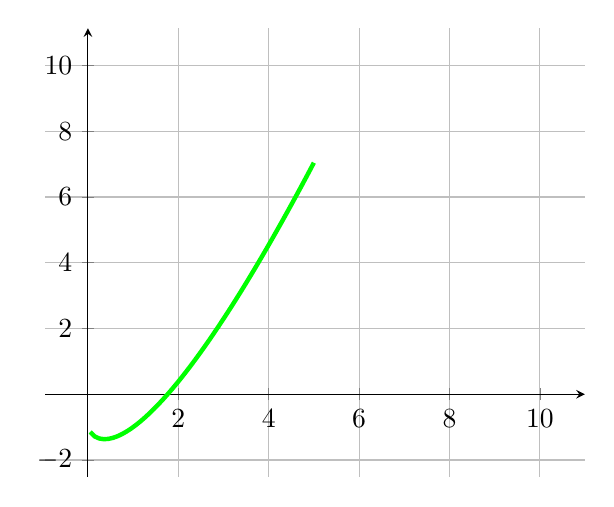
\begin{tikzpicture}
			\begin{axis}[grid=both,
				xmax=10,ymax=10,
				axis lines=middle,
				samples=100,
				enlargelimits]
				\addplot[green, ultra thick]  {x*ln(x)-1};
			\end{axis}
		\end{tikzpicture}
	\end{center}
	Quindi possiamo dire che 
	\begin{equation*}
		\exists ! \alpha \in \mathbb{R} \vert f(\alpha) = 0
	\end{equation*}
	Ci serve dare un \textbf{intervallo di localizzazione} della soluzione, ad esempio:
	\begin{align*}
		& f(1) = -1 \\
		& f(2) = 2 \log 2 -1 = log 4 -1 \\
		& \Rightarrow \alpha \in [1,2]
	\end{align*}
\end{example}

\subsection{Tecnica della separazione}
A partire da una funzione complessa, mi riconduco a funzioni più semplici e vedo dove si intercettano.
\begin{example}
	\label{example:non_linear_eq}
	Supponiamo di avere
	\begin{equation*}
		x \log x -1 = 0 \Leftrightarrow x \log x = 1 \Leftrightarrow \log x = \frac{1}{x}
	\end{equation*}
	Che sul grafico sono
	\begin{center}
		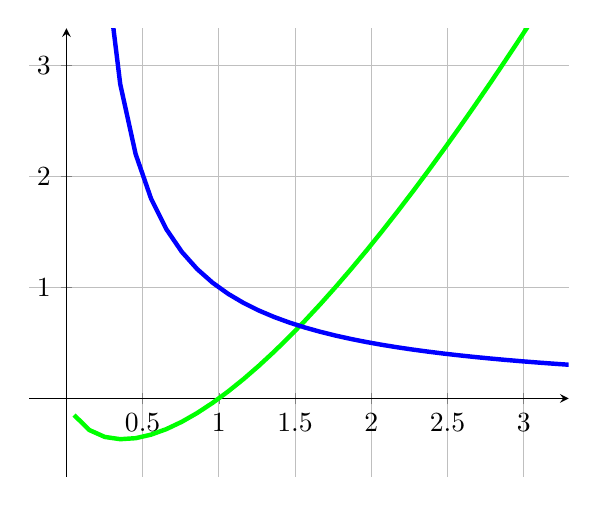
\begin{tikzpicture}
			\begin{axis}[grid=both,
				xmax=3,ymax=3,
				axis lines=middle,
				restrict x to domain=0:4,
				restrict y to domain=-2:4,
				samples=100,
				enlargelimits]
				\addplot[green, ultra thick]  {x*ln(x)};
				\addplot [blue, ultra thick] {1/x};
			\end{axis}
		\end{tikzpicture}
	\end{center}
	La studiamo:
	\begin{itemize}
		\item \textit{Dominio}: $f \in C^\infty(\mathbb{R}^+)$
		\item \textit{Limiti}:
		\begin{itemize}
			\item $\lim_{x\to 0^+} f(x) = -1$
			\item $\lim_{x\to +\infty} f(x) = +\infty$
		\end{itemize}
		\item Derivate:
		\begin{itemize}
			\item $f'(x)=\log x + 1 \geq 0 \Leftrightarrow \log x \geq -1 \Leftrightarrow x \geq \frac{1}{e}$
			\item $f''(x)=\frac{1}{x}>0 \quad \forall x \in \mathbb{R}^+$
		\end{itemize}
	\end{itemize}
\end{example}

\begin{example}
	Data la seguente funzione
	\begin{equation*}
		f(x) = e^x - 2x = 0 \Leftrightarrow e^x = 2x
	\end{equation*}
	È difficile usare il metodo della separazione perché l'intersezione non è facile da trovare. \\
	Usiamo quindi la soluzione grafica:
	\begin{itemize}
		\item \textbf{Dominio}: $\forall x \in \mathbb{R}$ che possiamo scrivere anche come $C^\infty (\mathbb{R})$
		\item \textbf{Limiti}:
		\begin{align*}
			& \lim_{x \to + \infty} e^x -2x = \lim_{x \to + \infty} e^x (1 - \frac{2x}{e^x}) = 0\\
			& \lim_{x \to - \infty} e^x -2x = + \infty\\
		\end{align*}
		\item \textbf{Derivata prima}: \begin{align*}
			& f'(x) = e^x -2 \\
			& f'(x) \geq 0 \Leftrightarrow e^x \geq 2 \Leftrightarrow x \geq \log 2
		\end{align*}
		\item \textbf{Derivata seconda}: $f''(x)=e^x$
	\end{itemize}
	\begin{center}
		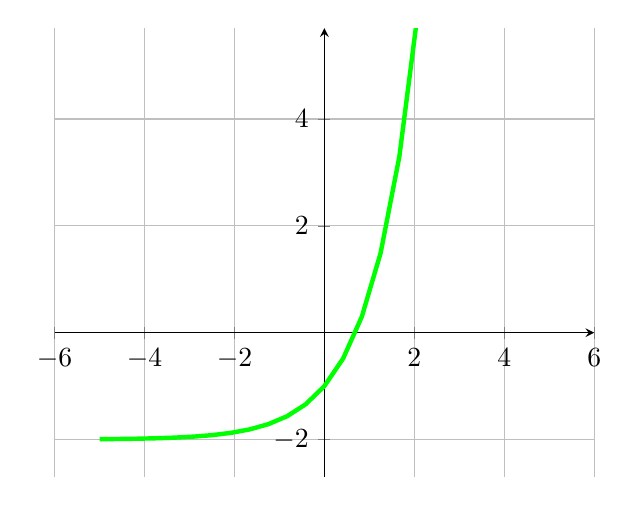
\begin{tikzpicture}
			\begin{axis}[grid=both,
				xmax=5,ymax=5,
				axis lines=middle,
				enlargelimits]
				\addplot[green, ultra thick]  {pow(e,x)-2};
			\end{axis}
		\end{tikzpicture}
	\end{center}	
	Calcoliamo adesso il valore in $\log 2$:
	\begin{equation*}
		f(\log 2) = e^{\log 2} - 2 \log 2 = 2-2 \log 2 = 2 (1-\log 2)
	\end{equation*}
\end{example}

\begin{example}
	Data la funzione:
	\begin{equation}
		f(x)= x^3 -6x +1 = 0
	\end{equation}
	In questo esempio abbiamo un polinomio e abbiamo quindi un'\textbf{equazione algebrica} di terzo grado. Quindi sappiamo il numero di soluzioni \textit{complesse}, nel nostro caso $3$. A noi però interessa il numero di soluzioni reali. Sapendo che quelle complesse devono andare sempre in coppia, potremo avere o due soluzioni complesse e una reale oppure tre soluzioni reali. Studiamo la funzione:
	\begin{itemize}
		\item \textbf{Dominio}: $\forall x \in \mathbb{R}$
		\item \textbf{Limiti}:
		\begin{align*}
			& \lim_{x \to + \infty} x^3 -6x +1 = + \infty\\
			& \lim_{x \to - \infty} x^3 -6x +1 = - \infty\\
		\end{align*}
		Sappiamo quindi che esiste sicuramente almeno un punto in cui la funzione vale $0$ per il teorema dell'esistenza degli zeri.
		\item \textbf{Derivata prima}: \begin{align*}
			& f'(x) = 3x^2-6 \\
			& f'(x) = 0 \Leftrightarrow x^2 = 2 \Leftrightarrow x = \pm \sqrt{2} \to x < -\sqrt{2} \land x > \sqrt{2}
		\end{align*}
		\item \textbf{Derivata seconda}: $f''(x)=6x \to f''(x) > 0 \Leftrightarrow x>0$
	\end{itemize}
	\begin{center}
		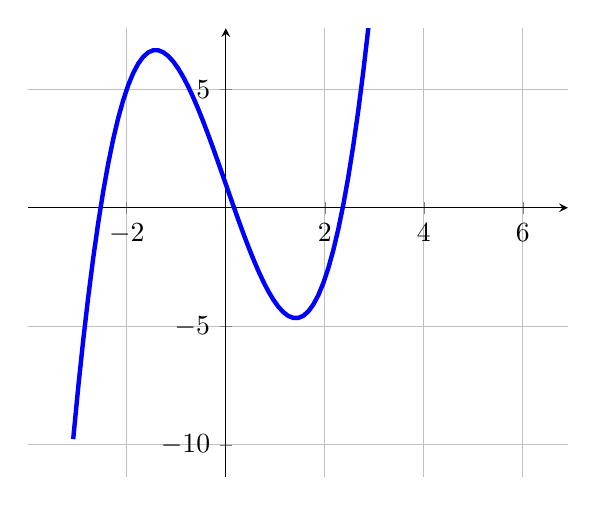
\begin{tikzpicture}
			\begin{axis}[grid=both,
				xmax=6,ymax=6,
				axis lines=middle,
				restrict x to domain=-4:4,
				restrict y to domain=-10:10,
				samples=100,
				enlargelimits]
				\addplot[blue, ultra thick] (x,x^3-6*x+1);
			\end{axis}
		\end{tikzpicture}
	\end{center}
	Quindi ci sono tre soluzioni reali, che possiamo localizzare come:
	\begin{align*}
		& \beta \in [0, \sqrt{2}]\\
		& \gamma \in [\sqrt{2}, 3]\\
		& \alpha \in [-3,-2]
	\end{align*}
\end{example}
\newpage
\subsection{Metodo di bisezione}
Vogliamo risolvere un'equazione $f(x)=0 \quad f:[a,b]\to \mathbb{R}$ che assumiamo essere \textit{continua} ($f \in C^0([a,b])$). Supponiamo poi che $f(a)f(b) < 0$, quindi la funzione assume valori discordi agli estremi. Questo implica, grazie al teorema di esistenza degli zeri, che $\exists \alpha \in [a,b] \:\vert f(\alpha)=0$, ovvero che esiste almeno un punto di intersezione con l'asse delle x.\\
Assumiamo che esista unico il punto di intersezione:
\begin{equation*}
	\exists ! \alpha \in [a,b] \:\vert\: f(x)=0
\end{equation*}
In questa situazione possiamo costruire diverse successioni che convergono ad $\alpha$ tramite il metodo di bisezione.
\begin{lstlisting}[language=MatLAB]
	a0 = a; b0=b; ya=f(a); yb=f(b);
	for k=1 : inf
		Ck = (a[k-1] + b[k-1])/2; % Calcolo il punto di mezzo dell'intervallo
		y = f(Ck);
		if(y * ya <= 0)
			ak = a[k-1]; bk=Ck; yb=y; % Qui la funzione e' discorde, mi sposto su questo intervallo
		else
			ak=Ck; bk=b[k-1]; ya=y; % Qui e' concorde, mi sposto sull'altro intervallo
		end
	end
\end{lstlisting}
Praticamente prendo il punto medio e controllo quale parte della funzione è concorde o discorde e mi sposto di conseguenza.
\begin{observation}
	Possiamo fare le seguenti osservazioni:
	\begin{enumerate}
		\item $a_k \leq b_k \quad \forall k$
		\item $\alpha \in [a_k, b_k] \quad \forall k$
		\item $b_k - a_k = \frac{b_{k-1}-a_{k-1}}{2} = \ldots = \frac{b_0 - a_0}{2^k}$
	\end{enumerate}
	che implicano:
	\begin{align*}
		& 0 \leq \lvert \alpha - a_k \rvert \leq b_k - a_k = \frac{b_0 - a_0}{2^k}\\
		& 0 \leq \lvert \alpha - b_k \rvert \leq b_k - a_k = \frac{b_0 - a_0}{2^k}\\
		& 0 \leq \lvert C_k  - \alpha \rvert \leq b_{k-1} - a_{k-1}\leq= \frac{b_0 - a_0}{2^k}
	\end{align*}
	e portando $k$ all'infinito, $a_k$, $b_k$ e $C_k$ tendono tutti ad $\alpha$.
\end{observation}

\begin{example}
	Supponiamo di voler risolvere
	\begin{equation*}
		f(x)=x-\cos x = 0
	\end{equation*}
	\newpage
	Proviamo prima con la \textbf{tecnica della separazione}:
	\begin{center}
		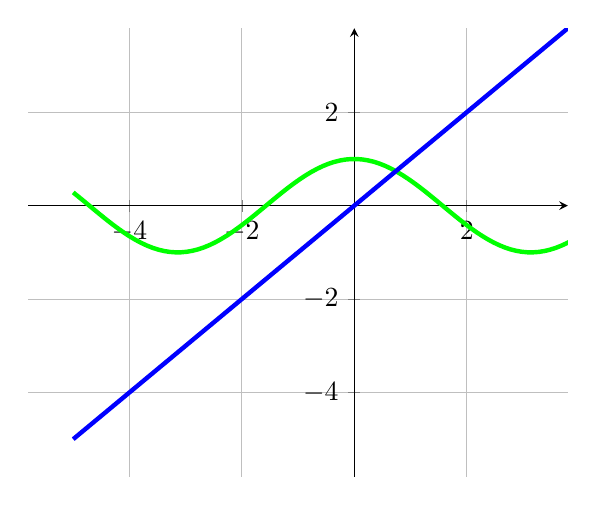
\begin{tikzpicture}
			\begin{axis}[grid=both,
				xmax=3,ymax=3,
				axis lines=middle,
				restrict x to domain=-5:5,
				restrict y to domain=-5:5,
				samples=100,
				enlargelimits]
				\addplot[green, ultra thick]  {cos(deg(x))};
				\addplot [blue, ultra thick] {x};
			\end{axis}
		\end{tikzpicture}
	\end{center}
	Osservando  attentamente notiamo che
	\begin{equation*}
		\exists ! \alpha \in [0,1]
	\end{equation*}
	poiché fuori da questo intervallo la funzione $x$ assume valori maggiori di $1$ o minori di $-1$ che non sono valori che può assumere la funzione $cos(x)$.\\
	Per poter usare il \textbf{metodo della bisezione} devo verificare che $f(x)$ sia continua e la sua monotonia.\\
	Come estremi per il metodo possiamo porre $[a,b]=[0,1]$.
	\begin{equation*}
		\lvert C_k - \alpha \rvert \leq \frac{b_0 - a_0}{2^k} \leq \epsilon
	\end{equation*}
	Posso a priori decidere la distanza dal mio numero finale facendo $\log_2 \frac{1}{\epsilon}$ passi.
\end{example}

\subsubsection{Approssimazione della radice}
Supponiamo di voler risolvere
\begin{equation*}
	x^2-2=0
\end{equation*}
Sappiamo che le soluzioni sono $x=\pm \sqrt{2}$ e che il grafico è:
\begin{center}
	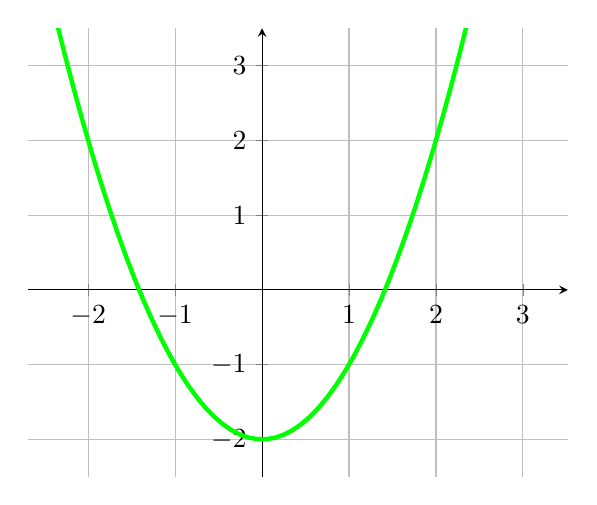
\begin{tikzpicture}
		\begin{axis}[grid=both,
			xmax=3,ymax=3,
			axis lines=middle,
			restrict x to domain=-5:5,
			restrict y to domain=-5:5,
			samples=100,
			enlargelimits]
			\addplot[green, ultra thick]  {x^2-2};
		\end{axis}
	\end{tikzpicture}
\end{center}
Il calcolatore non sa come calcolare $\sqrt{2}$, il modo migliore per farglielo fare è approssimare questa funzione con il metodo di bisezione nell'intervallo $[0,2]$.

\subsubsection{Svantaggi}
Questo metodo ha fondamentalmente due svantaggi:
\begin{itemize}
	\item Ha difficoltà ad essere esteso ai numeri \textbf{complessi}, ma per il nostro corso non ci riguarda
	\item Il \textbf{costo computazionale} è molto influenzato dal numero di valutazioni della funzioni che faccio e, dato che non conosco precisamente quali calcoli dovrà fare, potrebbe essere un problema. Nel metodo di bisezioni faccio una valutazione per passo e il numero di passi potrebbe essere elevato.
\end{itemize} 

\subsection{Metodo del punto fisso}
Questo metodo prevede di riscrivere il nostro problema come:
\begin{equation*}
	f(x) \Longleftrightarrow x = g(x)
\end{equation*}
\begin{example}
	Alcuni esempi:
	\begin{align*}
		&f(x)=0 \Longleftrightarrow x = x-f(x) \quad g(x) = x-f(x)\\
		& f(x)=0 \Longleftrightarrow x=x-\frac{f(x)}{h(x)} \quad g(x)=x-\frac{f(x)}{h(x)}
	\end{align*}
\end{example}
Poi si genera una successione da un punto iniziale:
\begin{equation*}
	\begin{cases}
		x_0 \in \mathbb{R} \\
		x_{\alpha +1} = g(x_\alpha)
	\end{cases}
\end{equation*}

\begin{example}
	\label{example:fixed_point}
	Partiamo dalla seguente equazione:
	\begin{equation*}
		x - \sqrt{x} = 0 \quad x \geq 0
	\end{equation*}
	Che posso riscrivere come:
	\begin{equation*}
		x = \sqrt{x} \Longleftrightarrow x^2 = x \Longleftrightarrow x = 0 \lor x=1
	\end{equation*}
	Notiamo come abbiamo ad esempio due possibili modi per scrivere l'equazione:
	\begin{align*}
		& x- \sqrt{x} = 0 \Longleftrightarrow x = \sqrt{x} \quad g_1(x)= \sqrt{x} \\
		& x- \sqrt{x} = 0 \Longleftrightarrow x^2 = x \quad g_2(x)=x^2
	\end{align*}
	Vediamo la successione generata da $g_1(x)$:
	\begin{equation*}
		\begin{cases}
			x_0 \in \mathbb{R}^+ \\
			x_{\alpha +1} = g_1(x_\alpha) = \sqrt{x_\alpha}
		\end{cases}
	\end{equation*}
	Che graficamente è
	\begin{center}
		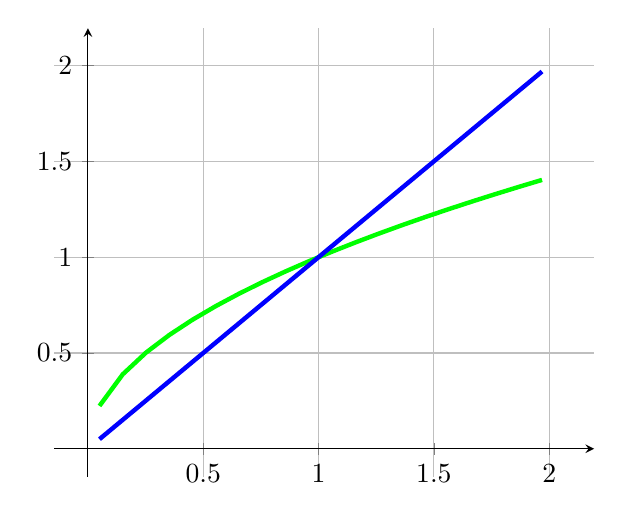
\begin{tikzpicture}
			\begin{axis}[grid=both,
				xmax=2,ymax=2,
				axis lines=middle,
				restrict x to domain=0:2,
				restrict y to domain=0:2,
				samples=100,
				enlargelimits]
				\addplot[green, ultra thick]  {sqrt(x)};
				\addplot[blue, ultra thick]  {x};
			\end{axis}
		\end{tikzpicture}
	\end{center}
	Con questa iterazione, se faccio i vari calcoli, da qualunque punto iniziale io scelga finirò alla soluzione $1$ (intersezione di $x$ e $\sqrt{x}$).\\
	Se scelgo invece la successione generata da $g_2(x)$, ottengo l'effetto contrario e trovo solo la soluzione $0$ quando parto da $0 < x_0 < 1 \lor -1 < x_0 < 0$, altrimenti la successione diverge a $+\infty$ per $x_0>1 \lor x_0 < -1$.
	\begin{center}
		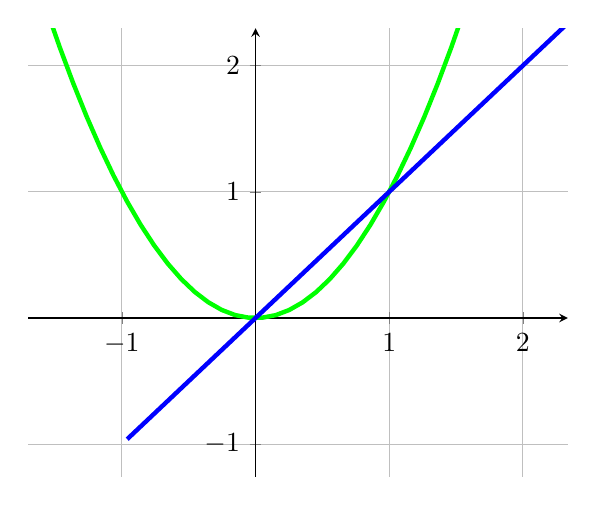
\begin{tikzpicture}
			\begin{axis}[grid=both,
				xmax=2,ymax=2,
				axis lines=middle,
				restrict x to domain=-2:3,
				restrict y to domain=-1:3,
				samples=100,
				enlargelimits]
				\addplot[green, ultra thick]  {x^2};
				\addplot[blue, ultra thick]  {x};
			\end{axis}
		\end{tikzpicture}
	\end{center}
\end{example}

\begin{theorem}[Teorema del punto fisso]
	Sia $g \in C^1([a,b])$, $\alpha \in (a,b)$ e $g(\alpha) = \alpha$ un \textbf{punto fisso}.\\
	\textit{Ipotesi}: se $\exists \rho >0 \:\vert\: \forall x \in [\alpha - \rho \alpha + \rho]=I_\alpha \geq [a,b]$ si ha che $\lvert g(x) \rvert < 1$.\\
	\textit{Tesi}: allora $\forall x_0 \in I_\alpha$ la successione generata dal metodo $x_{k+1} = g(x_k)$ soddisfa le seguenti proprietà:
	\begin{itemize}
		\item $x_= \in I_\alpha \quad \forall k$
		\item $x_k \to \alpha$
	\end{itemize}
\end{theorem}

\begin{observation}
	È importante nel precedente teorema che l'intervallo $[a,b]$ sia centrato per garantire che da qualunque punto si inizi si riduca la distanza dal punto fisso senza però uscire dall'intervallo.
\end{observation}

\begin{demostration}
	Sappiamo che se $g(x)$ è continua allora anche $\lvert g'(x) \rvert$ è continua. Per il \textbf{teorema di Weirstrass} sappiamo che una funzione continua su un intervallo limitato ammette \textit{massimo}, nel nostro caso $\lambda < 1$. \\
	Dimostriamo per induzione che $x_0 \in I_\alpha \Rightarrow \lvert x_k -\alpha \rvert \leq \lambda^k \rho \quad \forall k \geq 0$:
	\begin{itemize}
		\item \textit{Passo base}: per $k=0$ abbiamo che: 
		\begin{equation*}
			\lvert x_0 - \alpha \rvert \leq \lambda^0 \rho = \alpha
		\end{equation*}
		che è vero per le ipotesi: $x_0 \in I_\alpha$.
		\item \textit{Passo induttivo}: posso scrivere:
		\begin{equation*}
			\lvert x_{k+1} - \alpha \rvert = \lvert g(x_k) - g(\alpha) \rvert = \lvert g'(\psi k)(x_k - \alpha) \rvert = \lvert g'(\psi k) \rvert  \lvert x_k - \alpha \rvert \leq \lambda \lambda^k \rho = \lambda ^ {k+1} \rho
		\end{equation*}
	\end{itemize}
\end{demostration}

\begin{example}
	Partiamo dalla funzione dell'esempio \ref{example:fixed_point}, in particolare da $g_1$:
	\begin{equation*}
		g'_1(x) = \frac{1}{2 \sqrt{x}} \Longrightarrow \lvert g'_1(x) \rvert = \lvert \frac{1}{2} \frac{1}{\sqrt{x}} \rvert = \frac{1}{2 \sqrt{x}}
	\end{equation*}
	Vediamo dove il suo modulo è minore di $1$:
	\begin{equation*}
		\frac{1}{2 \sqrt{x}} < 1 \Leftrightarrow 2 \sqrt{x} > 1 \Leftrightarrow \sqrt{x} > \frac{1}{2} \Leftrightarrow x> \frac{1}{4}
	\end{equation*}
	Quindi comunque si scelga un intervallo centrato in $1$ tale che $x>\frac{1}{4}$ (al massimo potrò avere $[\frac{1}{4}, \frac{5}{4}]$) allora la successione converge.\\
	Vediamo la funzione $g_2$:
	\begin{equation*}
		g'_2(x) = 2x \Longrightarrow \lvert g'_2(x) \rvert = \lvert 2x \rvert = 2 \lvert x \rvert
	\end{equation*}
	Vediamo dove il suo modulo è minore di $1$:
	\begin{equation*}
		2 \lvert x \rvert < 1 \Leftrightarrow \lvert x \rvert < \frac{1}{2}
	\end{equation*}
	Quindi comunque si scelga un intervallo centrato in $0$ tale che $x$ è compreso tra $-\frac{1}{2}$ e $\frac{1}{2}$, allora la successione converge.
\end{example}

\begin{theorem}
	Prendiamo $g \in C^1([a,b]) \quad g(\alpha)=\alpha \quad \alpha \in (a,b)$. \\
	Se $\lvert g'(\alpha) \rvert < 1$, prendiamo $h(x) = \lvert g'(x) \rvert -1$ quindi:
	\begin{equation*}
		h(\alpha) = \lvert g'(\alpha) \rvert -1 < 0 \Rightarrow \exists [\alpha-\rho, \alpha + \rho] = I_\alpha \:\vert\: \forall x \in I_\alpha \quad h(x)<0 \Leftrightarrow \lvert g'(x) \rvert <1
	\end{equation*}
	Quindi posso dire che $\alpha$ è \textbf{punto attrattivo} (se parto vicino ad $\alpha$ convergo su di esso, esiste un intorno e c'è convergenza locale). Altrimenti è \textbf{punto repulsivo}. Se è uguale, allora è \textbf{neutrale}.
\end{theorem}

\begin{example}
	Prendiamo la funzione
	\begin{equation*}
		f(x) = e^{-x} - x = 0
	\end{equation*}
	\begin{enumerate}
		\item Utilizziamo il metodo di separazione grafica per determinare che esiste unica la soluzione:
		\begin{equation*}
			e^{-x} - x = 0 \Leftrightarrow e^{-x} = x
		\end{equation*}
		\begin{center}
			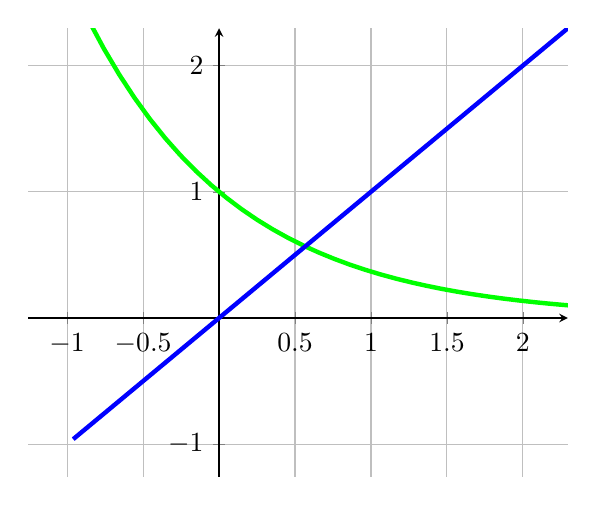
\begin{tikzpicture}
				\begin{axis}[grid=both,
					xmax=2,ymax=2,
					axis lines=middle,
					restrict x to domain=-2:3,
					restrict y to domain=-1:3,
					samples=100,
					enlargelimits]
					\addplot[green, ultra thick]  {e^(-x)};
					\addplot[blue, ultra thick]  {x};
				\end{axis}
			\end{tikzpicture}
		\end{center}
		E ho trovato un intervallo di separazione $\alpha \in [0, 1]$.
		\item Consideriamo il metodo iterativo
		\begin{equation*}
			x_{k+1} = e^{-x_k} \quad k \geq 0
		\end{equation*}
		\begin{itemize}
			\item Dire se l'intervallo è localmente convergente. Sappiamo che 
			\begin{equation*}
				g'(x)=-e^{-x} \Rightarrow \lvert g'(x) \rvert = e^{-x}
			\end{equation*}
			quindi
			\begin{equation*}
				e^{-x} < 1 \Leftrightarrow -x < 0 \Leftrightarrow x >0
			\end{equation*}
			e posso dire che $\lvert g'(\alpha)  \rvert< 1$ e quindi il metodo è \textbf{localmente convergente}.
			\item Si dica come scegliere un punto iniziale a partire dal quale il metodo converge. Per localizzare $\alpha$, utilizzo il metodo di bisezione:
			\begin{equation*}
				x=\frac{1}{2} \Rightarrow g(\frac{1}{2}) = \frac{1}{\sqrt{e}} > \frac{1}{2}
			\end{equation*}
			Quindi posso scegliere $1$ perché ho abbastanza spazio dall'altro lato per centrare l'intervallo in $\alpha$.
		\end{itemize}
	\end{enumerate}
\end{example}
\newpage
\begin{example}
	Prendiamo la funzione dell'esempio \ref{example:non_linear_eq} e vediamo che
	\begin{equation*}
		\alpha \in [1,2]
	\end{equation*}
	Consideriamo due metodi iterativi:
	\begin{itemize}
		\item
		\begin{equation*}
			x_{k+1} = \frac{1}{\ln {x_k}} \quad k \geq 0
		\end{equation*}
		\item 
		\begin{equation*}
			x_{k+1} = e^{\frac{1}{x_k}} \quad k \geq 0
		\end{equation*}
	\end{itemize}
	Verifichiamo le derivate:
	\begin{itemize}
		\item 
		\begin{equation*}
			g'(x) = \frac{- \frac{1}{x}}{\ln ^ 2 {x}} \Rightarrow \lvert \frac{- \frac{1}{x}}{\ln ^ 2 {x}} \rvert  = \frac{1}{x \ln^2 x}
		\end{equation*}
		La valuto in $\alpha$ tenendo a mente che è punto fisso ($\alpha = \frac{1}{\alpha}$):
		\begin{equation*}
			\lvert g'(\alpha)\rvert = \frac{1}{\alpha \ln ^2 \alpha} = \frac{\alpha^2}{\alpha} = \alpha > 1
		\end{equation*}
		E quindi per questo metodo è un \textbf{punto repulsivo}.
		\item \begin{equation*}
			g'(x) = e^\frac{1}{x}(-\frac{1}{x^2})
		\end{equation*}
		La valuto in $\alpha$:
		\begin{equation*}
			\lvert g'(\alpha) \rvert = e^\frac{1}{\alpha}(-\frac{1}{\alpha^2}) = \frac{1}{\alpha} < 1
		\end{equation*}
		E quindi per questo metodo è un \textbf{punto attrattivo}.
	\end{itemize}
\end{example}

\subsection{Metodo delle tangenti}
In questo metodo (anche chiamato \textit{di Newton}) si utilizza la \textbf{tangente} per approssimare il punto, in quanto è una buona approssimazione locale, e poi si interseca questa con l'asse delle $x$.\\
Partiamo da un punto:
\begin{equation*}
	P=(x_0,f(x_0))
\end{equation*}
di cui posso scrivere la retta tangente come:
\begin{equation*}
	y-f(x_0)=f'(x_0)(x-x_0)
\end{equation*}
\begin{note}
	La funzione per questo metodo deve essere non solo continua ma anche \textbf{derivabile}. Per ottenere quindi maggiore precisione dobbiamo porre più restrizioni sulla funzione:
	\begin{equation*}
		f \in C^1([a,b])
	\end{equation*}
\end{note}
\noindent Intersechiamo la tangente con l'asse delle $x$:
\begin{equation*}
	\begin{cases}
		y-f(x_0)=f'(x_0)(x-x_0) \\
		y=0
	\end{cases} \to 
	x_1-x_0 = -\frac{f(x_0)}{f'(x_0)} \Rightarrow x_1 = x_0 -\frac{f(x_0)}{f'(x_0)}
\end{equation*}
\begin{note}
	Diventa quindi necessario aggiungere la seguente restrizione:
	\begin{equation*}
		f'(\alpha) \neq 0
	\end{equation*}
\end{note}

\subsubsection{Convergenza locale}
Il metodo delle tangenti può essere visto come un metodo di iterazione funzionale in cui:
\begin{equation*}
	x_{k+1}=g(x_k) \quad g(x)=x-\frac{f(x)}{f'(x)}
\end{equation*}
Verifichiamo che sia \textbf{localmente convergente}:
\begin{align*}
	& g'(x)=1 - \frac{f'(x) \cdot f'(x) - f''(x) \cdot f(x)}{(f'(x))^2} = \frac{f''(x) \cdot f(x)}{(f'(x))^2} \\
	& \lvert g'(\alpha) \rvert = \lvert  \frac{f''(\alpha) \cdot f(\alpha)}{(f'(\alpha))^2} \rvert = 0 < 1
\end{align*}
\begin{note}
	Questo ci porta ad aggiungere un'altra restrizione alla funzione, ovvero che sia derivabile due volte.
	\begin{equation*}
		f \in C^2([a,b])
	\end{equation*}
\end{note}

\begin{example}
	Data la funzione
	\begin{equation*}
		f(x)=x^2
	\end{equation*}
	che si noti non rispettare $f'(\alpha)\neq 0$. \\
	Scriviamo il metodo delle tangenti:
	\begin{equation*}
		x_{k+1}=x_k - \frac{x_k^2}{2x_k}=x_k-\frac{1}{2}x_k=\frac{1}{2}x_k
	\end{equation*}
	e quindi
	\begin{equation*}
		x_k=\bigg(\frac{1}{2}\bigg)^k x_0
	\end{equation*}
	Vediamo quindi che può convergere anche se non viene rispettata quella clausola. Noi comunque la manteniamo per semplificarci i calcoli.
\end{example}

\subsubsection{Convergenza lineare}
Supponiamo di avere una successione che converge ad $\alpha$:
\begin{equation*}
	x_k \to \alpha \quad x_n \neq \alpha \forall n
\end{equation*}
Vediamo che converge linearmente se:
\begin{equation*}
	\lim_{n \to \infty} \lvert \frac{x_{k+1}-\alpha}{x_{n}-\alpha}\rvert = l \quad 0 < l < 1
\end{equation*}
Questo significa che ad ogni passo l'errore si riduce di un fattore $l$.\\
Se assumiamo $l=\frac{1}{2}$ vediamo che, data una tolleranza $\epsilon$, il numero di passi è:
\begin{equation*}
	\bigg(\frac{1}{2}\bigg)^n \leq \epsilon \Leftrightarrow n \log \frac{1}{2} \leq \log \epsilon \Leftrightarrow -n \leq \log \epsilon \Leftrightarrow n \geq \log \frac{1}{\epsilon}
\end{equation*}

\subsubsection{Convergenza quadratica}
Una successione converge almeno quadraticamente se
\begin{equation*}
	\lim_{n \to \infty} \frac{\lvert x_{k+1}-\alpha \rvert}{\lvert x_{n}-\alpha \rvert ^2} = l \in \mathbb{R}
\end{equation*}
Se assumiamo $l=1$ , data una tolleranza $\epsilon$, il numero di passi da fare è:
\begin{equation*}
	\bigg(\frac{1}{2}\bigg)^{2^n} \leq \epsilon \Leftrightarrow -2^n \leq \log \epsilon \Leftrightarrow 2^n \geq \log \frac{1}{\epsilon} \Leftrightarrow n \geq \log \log \frac{1}{\epsilon}
\end{equation*}
Quindi con un metodo che converge quadraticamente, anche nel caso in cui abbiamo un fattore di riduzione peggiore rispetto che ad un metodo lineare, abbiamo un numero comunque ridotto di passi da eseguire. 
\begin{demostration}[Convergenza quadratica del metodo delle tangenti]
	\begin{align*}
		& 0=f(\alpha)=f(x_n)+f'(x_n)(\alpha-x_n)+f''(\psi_n)(x_n-\alpha)^2 \quad \psi_n \in [x_n,\alpha] \\
		& -\frac{f(x_n)}{f'(x_n)} = (\alpha - x_n) + \frac{f''(\psi_n)(x_n-\alpha)^2}{2f'(x_n)} \\
		& = \alpha + \frac{f''(\psi_n)(x_n-\alpha)^2}{2f'(x_n)} \\
		& \bigg\lvert \frac{x_{n+1}-\alpha}{(x_n-\alpha)^2}\bigg\rvert = \bigg\lvert \frac{f''(\psi_n)}{2f'(\psi_n)}\bigg\rvert \to \frac{\lvert f'(\alpha)\rvert}{\lvert 2 f'(\alpha)\rvert}=l\in \mathbb{R}
	\end{align*}
\end{demostration}

\begin{example}
	Data la funzione:
	\begin{equation*}
		e^x+x+2=0
	\end{equation*}
	Se studiamo la funzione vediamo:
	\begin{itemize}
		\item \textit{Dominio}: $f \in C^\infty(\mathbb{R})$
		\item \textit{Limiti}:
		\begin{itemize}
			\item $\lim_{x \to + \infty}f(x) = + \infty$
			\item $\lim_{x \to - \infty}f(x) = - \infty$
		\end{itemize}
		\item \textit{Derivate}:
		\begin{itemize}
			\item $f'(x) = e^x+1 \geq 0 \quad \forall x \in \mathbb{R}$
			\item $f''(x) = e^x \geq 0 \quad \forall x \in \mathbb{R}$
		\end{itemize}
	\end{itemize}
		\begin{center}
		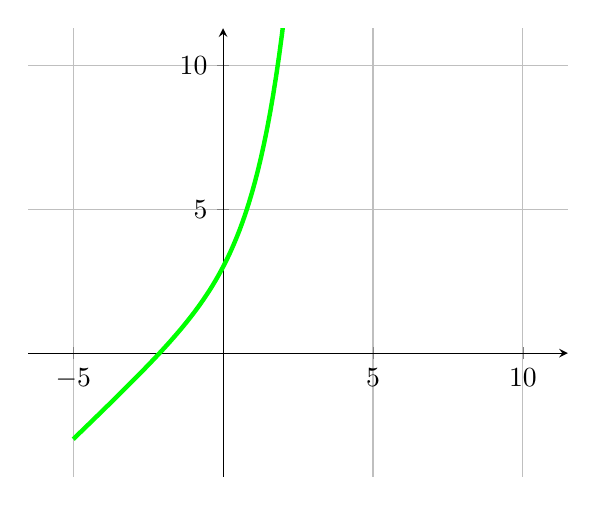
\begin{tikzpicture}
			\begin{axis}[grid=both,
				xmax=10,ymax=10,
				axis lines=middle,
				restrict x to domain=-20:20,
				restrict y to domain=-20:20,
				samples=100,
				enlargelimits]
				\addplot[green, ultra thick]  {e^x+x+2};
			\end{axis}
		\end{tikzpicture}
	\end{center}
	Possiamo dire che:
	\begin{equation*}
		\exists ! \alpha \in \mathbb{R} \:\vert\: f(\alpha)=0 \quad f \in C^2(\mathbb{R}) \quad f'(\alpha)\neq 0
	\end{equation*}
	e che quindi questo metodo è \textbf{localmente convergente}.
\end{example}

\begin{example}
	Data la funzione:
	\begin{equation*}
		xa-1=0 \quad a \in \mathbb{R} \quad a \neq 0
	\end{equation*}
	Possiamo facilmente vedere che
	\begin{equation*}
		x=\frac{1}{a}
	\end{equation*}
	Con un metodo lineare converge in un passo. Proviamo però a vederla come:
	\begin{equation*}
		a=\frac{1}{x} \Leftrightarrow \frac{1}{x}-a=0
	\end{equation*}
	e applichiamo il metodo delle tangenti:
	\begin{equation*}
		x_{k+1}=x_k + \frac{\big(\frac{1}{x_k} - a\big)}{\frac{1}{x_k^2}} = x_k + x_k^2 \cdot \bigg(\frac{1}{x_k} - a\bigg) = 2x_k-ax_k^2
	\end{equation*}
	Che ha bisogno di un numero di passi maggiore. Però non fa divisioni ma solamente prodotti e addizioni. Questo nei primi calcolatori che avevano solo addizioni, sottrazioni e moltiplicazioni, era il metodo che veniva utilizzato per approssimare le divisioni.
\end{example}

\begin{example}
	Data la funzione dell'esercizio \ref{example:non_linear_eq}. Vediamo che se partiamo con il metodo delle tangenti da $\frac{1}{e}$, la successione diverge. Se invece si sceglie un valore di partenza tra $0$ e $\frac{1}{e}$, la successione passa dall'aritmetica reale a quella complessa dato che la macchina gestisce anche i logaritmi di numeri negativi.
\end{example}